% vim: spell spelllang=en:
%! TEX root = **/00-main.tex

%Motivation of the work and general description of the problem to be analyzed (max one page)

\section{Motivation}%
\label{sec:motivation}

During the last decade \airbnb has become a disrupting force it the
short-term rental market, especially when geared towards tourism, and
increasingly, persuaded by the easy and painless sign up process, people
are uploading their properties in order to earn extra cash, or even becoming
their main source of income.

\begin{figure}[H]
    \centering
    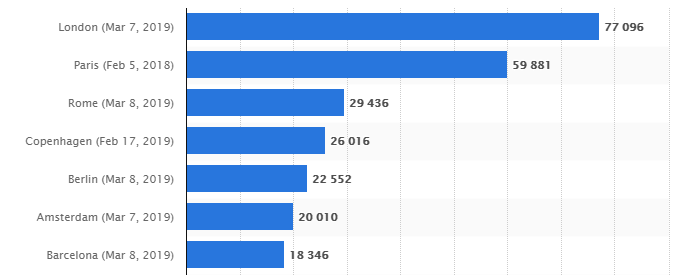
\includegraphics[width=0.6\linewidth]{images/listingplot}
    \caption{\airbnb 2019 new listings}%
    \label{fig:airbnblistingsPlot.PNG}
\end{figure}

When looking at the number of \airbnb listings, we found out that Barcelona,
with 18,346 listings in 2019, ranked as the seventh European
city~\cite{europe2019}. As well as the first among Spanish cities. This suggests
that Barcelona is one of the biggest \airbnb markets and therefore an
interesting way to explore it's revolutionary business model.

Furthermore a study realised in 2013 found out hat \airbnb generated \$175
million in economic activity in one year in Barcelona and supported 4,310
jobs~\cite{economy}. As many more users have listed rentals since then, we
can only expect that nowadays the amount of jobs and revenue it brings to
the city have only increased.

\begin{figure}[H]
    \centering
    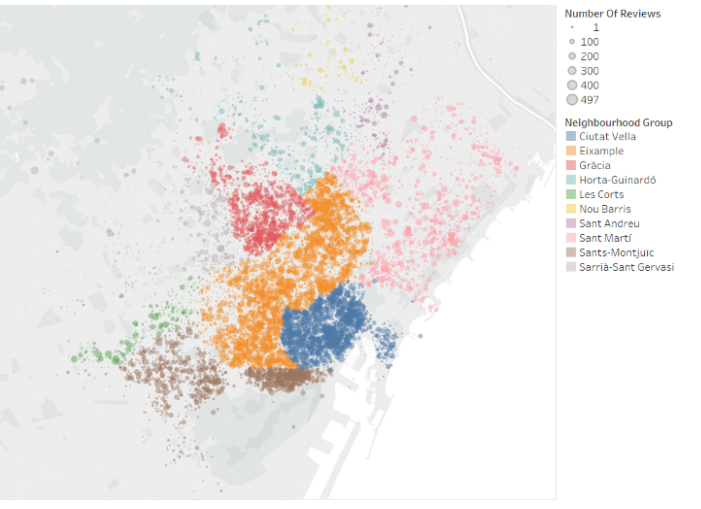
\includegraphics[width=0.5\linewidth]{images/airbnbMap}
    \caption{\airbnb map}%
    \label{fig:airbnbMap.PNG}
\end{figure}

We are specially interested in analysing what makes a successful \airbnb rental.
One of the focus of the project will be to analyse whether or not factors
such as price, availability or neighbourhood impact whether or not the final
user review is positive or negative.
